
\section{Labeling Function: {\normalfont\normalsize For your analysis, you may focus on a subset of the 58 classes provided.}}
\label{sec:Labeling Function}

For subtasks b.) and c.), we focused primarily on the following randomly selected subset classes: Airplane, Bird Chirp, Power Drill, Cowbell, Siren, Trumpet, and Rooster Crow.

\subsection{Assess how accurately the applied labeling functions capture the intended classes. Do the mapped classes correspond well to the free-text annotations? Are the labeled events clearly audible within the indicated time regions?}
\label{sec:Labeling Function:a}
To evaluate the accuracy of the applied labeling function, the free text annotations were analyzed by applying an algorithm that counted the frequency of semantically meaningful words in each annotation (Tabel ~\ref{tbl:1}).
The resulting list of most common words per label clearly showed that the labeling function captured the intended classes with a high accuracy; e.g. all words related to dogs (dog, barking, growling) were clearly captured under a single label. Indicating that the labeled events are clearly audible within the indicated time regions. This was further proven by checking random samples that aligned with the given labels. \\
This was further confirmed by laying a random selection of labels over a clustered down-projection of the audio features (see section 1.c.).




\begin{table}[ht]
\centering
\caption{Top 3 Annotation Keywords per Label}
\label{tab:keyword_summary_dots_count}
\begin{tabular}{l l r l r l r r}
\toprule
\textbf{Class} & \textbf{Keyword 1} & \textbf{Count} & \textbf{Keyword 2} & \textbf{Count} & \textbf{Keyword 3} & \textbf{Count} & \textbf{Total per Label} \\
\midrule
\textbf{Alarm} & alarm & 359 & beeps & 110 & clock & 78 & 547 \\
\textbf{Beep/Bleep} & beep & 251 & beeps & 231 & beeping & 193 & 675 \\
\textbf{Car} & car & 741 & engine & 333 & driving & 179 & 1253 \\
\textbf{Speech} & speaking & 1166 & talking & 602 & man & 608 & 2376 \\
\textbf{Hammer} & hammer & 259 & hammering & 147 & metallic & 98 & 504 \\
\textbf{Siren} & siren & 351 & police & 80 & ambulance & 61 & 492 \\
\textbf{Bell} & bell & 655 & rings & 442 & ringing & 231 & 1328 \\
\textbf{Shout} & shouting & 187 & loudly & 208 & screams & 130 & 525 \\
\midrule
\textbf{\dots} & \dots & \dots & \dots & \dots & \dots & \dots & \dots \\
\midrule
\textbf{Hiccup} & hiccups & 36 & baby & 19 & high-pitched & 17 & 72 \\
\textbf{Jackhammer} & jackhammer & 121 & construction & 67 & loud & 46 & 234 \\
\textbf{Sewing Machine} & sewing & 78 & machine & 78 & mechanical & 20 & 176 \\
\textbf{Cowbell} & cowbell & 65 & cowbells & 44 & ringing & 31 & 140 \\
\textbf{Pig Oink} & pig & 127 & grunts & 72 & snorts & 23 & 222 \\
\textbf{Chainsaw} & chainsaw & 232 & running & 48 & cutting & 31 & 311 \\
\textbf{Washing Machine} & washing & 176 & machine & 176 & water & 23 & 375 \\
\textbf{Power Saw} & saw & 138 & cutting & 72 & circular & 43 & 253 \\
\bottomrule
\label{tbl:1}
\end{tabular}
\end{table}



\subsection{Which audio features appear most useful for distinguishing between the classes of interest? }
\label{sec:Labeling Function:b}

In order to answer this question, we first of all randomly collected 1000 frames from the dataset (which represents a collection of all frames from all files) per class where it is positive, resulting in a total of around 7000 frames (a bit less, since some frames contain multiple of the classes). For each frame, we additionally include the previous and next two frames as context length by simply concatenating them with the features from the central frame (in temporal order). Each class therefore has 1000 vectors of shape 5 * 942 = 4710, where 942 represents the summed number of dimensions for all features.

For each class, we then estimated the Mutual Information between the label vector and all features dimensions. For each feature, we then calculated the average Mutual Information over all feature dimension corresponding to it. This gives us a measure for how informative the feature generally is for predicting the label correctly, which also captures nonlinear relationships. We then normalized the values per label, resulting in the first plot of (Figure ~\ref{fig:1_FI}). However, since this approach cannot capture effects features only have in combination with one another, we also tried fitting a simple Random Forest Classifier on the data and extracted its feature importances, resulting in the second plot of (Figure ~\ref{fig:1_FI}).

\begin{figure}[htbp]
  \centering
  \begin{subfigure}[b]{0.49\textwidth}
    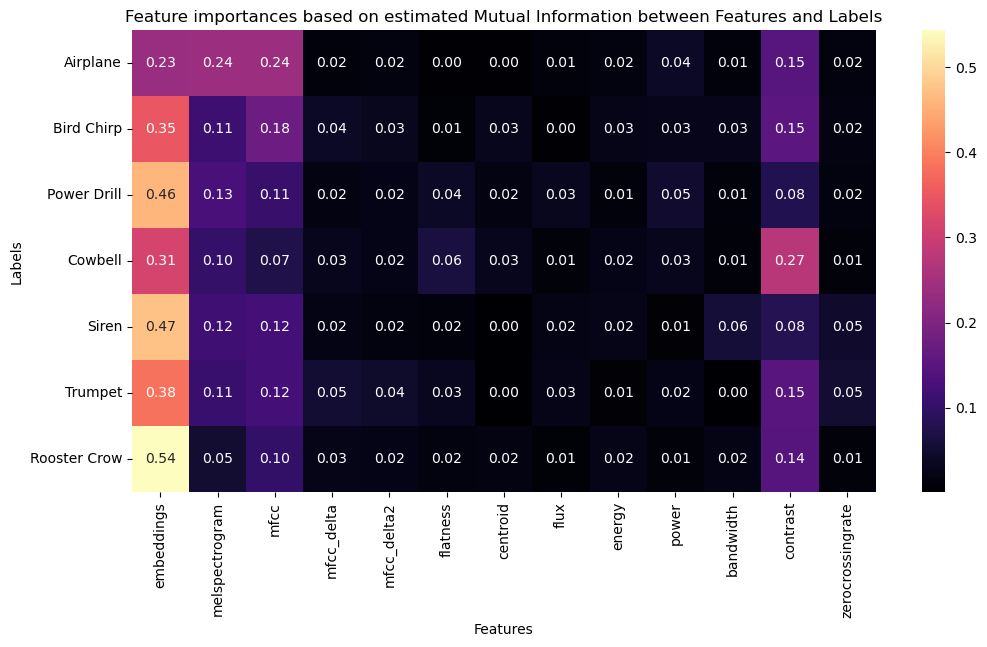
\includegraphics[width=\textwidth, height=5cm]{figs/1_MI.png}
  \end{subfigure}
  \hfill
  \begin{subfigure}[b]{0.49\textwidth}
    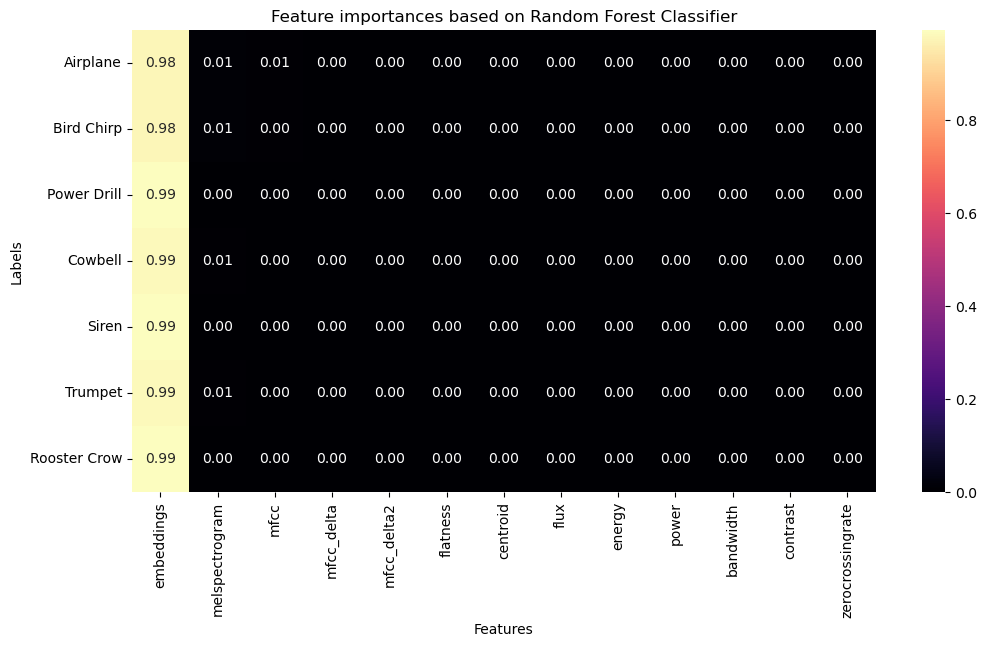
\includegraphics[width=\textwidth, height=5cm]{figs/1_RF.png}
  \end{subfigure}
  \caption{Estimated feature importances as by Mutual Inforamation and Random Forest methods.}
  \label{fig:1_FI}
\end{figure}

The features 'embeddings', 'melspectrogram', 'mfcc' and 'contrast' all seem to be pretty useful according to our Mutual Information graphic, with 'embeddings' being the most important one. However, the fact that the Random Forest almost exclusively relies on the embeddings might suggest heavy correlations between them and the other features. Which does make sense, considering many of the other features are usually used for creating such audio embeddings.


\subsection{How well do the chosen audio features group according to the discretized class labels? Do samples of the same class form tight clusters?}
\label{sec:Labeling Function:c}
Using the four features mentioned above, we reduced the high-dimensional data to two dimension using T-SNE and plotted the results in (Figure ~\ref{fig:1_TSNE}). Note that for examples corresponding to more than one of the classes, we randomly chose one for coloring.

\begin{figure}[htbp]
    \centering
    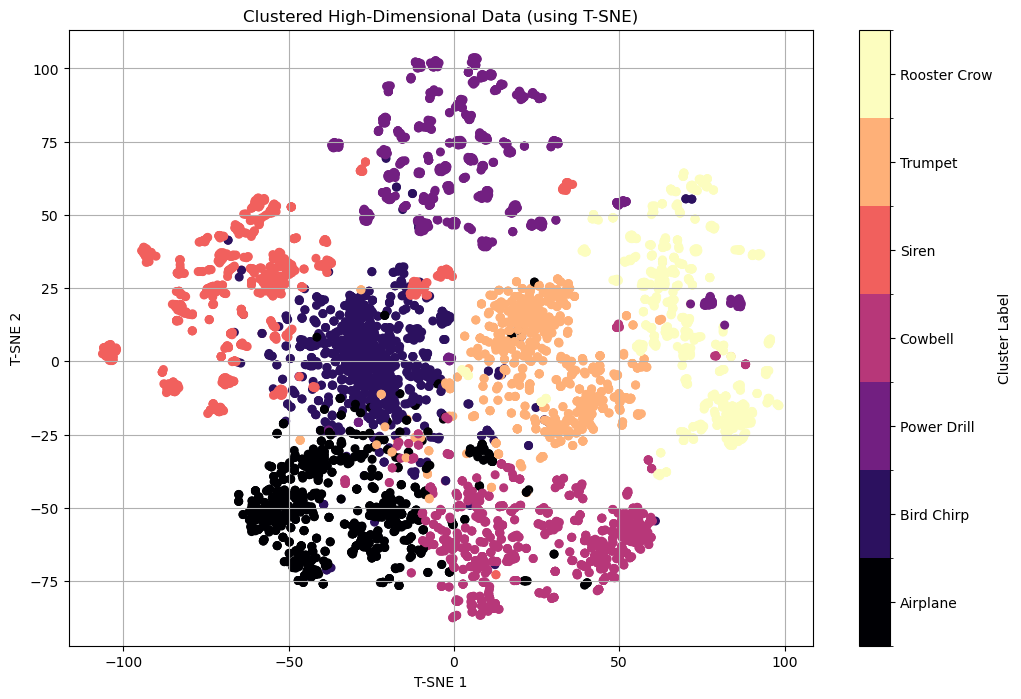
\includegraphics[width=0.5\linewidth, height=5cm]{figs/1_TSNE.png}
    \caption{Downprojected examples using selected features and their class correspondences.}
    \label{fig:1_TSNE}
\end{figure}

Overall, the results look very reasonable. Clusters are identifiable and examples within mostly have the same attributed class. Some overlaps are of course inevitable, considering the relatively high complexity of the dataset. 